\documentclass{workbook}

\newcommand{\copyrightdate}{2025}

\usepackage{ifxetex}
\usepackage[utf8]{inputenc}
\usepackage{hyperref}
\usepackage{hyperxmp} % Embed meta data into the PDF
\hypersetup{%
	hidelinks=true,
	linkcolor = {0 0 1},
	% Metadata to be embedded by hyperxmp
	pdftitle={Calculus II (\jobname)},
	pdfauthor={Jason Siefken, Geoff McGregor, Arman Pannu},
	pdfauthortitle={Author},
	pdfcopyright={Copyright (C) \copyrightdate, Jason Siefken, Geoff McGregor, Arman Pannu},
	pdfsubject={Calculus 2 textbook/workbook},
	pdfkeywords={calculus 2},
	pdfurl={https://github.com/siefkenj/MAT187-2025/},
	pdflicenseurl={https://creativecommons.org/licenses/by-sa/4.0/},
}

%%%
% import all needed packages and macros
%%%
\usepackage[yyyymmdd]{datetime}
\input{common/preamble.tex}

\usepackage{breqn}

\usepackage{pdfrender} % For text title


%%%
% Set up the footers to have the correct copyright notices
%%%

\fancypagestyle{siefken}{%
	\rfoot{\footnotesize\it \copyright\,Geoff McGregor, Arman Pannu \& Jason Siefken, \copyrightdate \ \makebox(30,5){\includegraphics[height=1.2em]{by-sa.pdf}}}
	\lfoot{}
	\renewcommand{\headrulewidth}{0pt}
}


%%
% Allow hiding of environments
%%
\usepackage{environ}% http://ctan.org/pkg/environ
\makeatletter
\newcommand{\voidenvironment}[1]{%
  \expandafter\providecommand\csname env@#1@save@env\endcsname{}%
  \expandafter\providecommand\csname env@#1@process\endcsname{}%
  \@ifundefined{#1}{}{\RenewEnviron{#1}{}}%
}
\makeatother
% allow pagebreaks that only display in `standard` mode
\newcommand{\displayonlynewpage}{\begin{displayonly}\newpage\end{displayonly}}
% allow pagebreaks that only display in `book` mode
\newcommand{\bookonlynewpage}{\begin{bookonly}\newpage\end{bookonly}}


%
% Set up the three render modes: standard, instructor, and solutions.
% These render with varying amounts of extra data (like solutions and notes)
%
\newtoggle{instructor}
\newtoggle{standard}
\newtoggle{solutions}
\newtoggle{book}
\newtoggle{slides}
\newtoggle{slideswhite}
\newcommand{\setinstructor}{
	\toggletrue{instructor}
	\togglefalse{standard}
	\togglefalse{solutions}
	\togglefalse{book}
	\togglefalse{slides}
	\togglefalse{slideswhite}
}
\newcommand{\setstandard}{
	\togglefalse{instructor}
	\toggletrue{standard}
	\togglefalse{solutions}
	\togglefalse{book}
	\togglefalse{slides}
	\togglefalse{slideswhite}
}
\newcommand{\setsolutions}{
	\togglefalse{instructor}
	\togglefalse{standard}
	\toggletrue{solutions}
	\togglefalse{book}
	\togglefalse{slides}
	\togglefalse{slideswhite}
}
\newcommand{\setbook}{
	\togglefalse{instructor}
	\togglefalse{standard}
	\togglefalse{solutions}
	\toggletrue{book}
	\togglefalse{slides}
	\togglefalse{slideswhite}
}
\newcommand{\setslides}{
	\togglefalse{instructor}
	\togglefalse{standard}
	\togglefalse{solutions}
	\togglefalse{book}
	\toggletrue{slides}
	\togglefalse{slideswhite}
}
\newcommand{\setslideswhite}{
	\togglefalse{instructor}
	\togglefalse{standard}
	\togglefalse{solutions}
	\togglefalse{book}
	\togglefalse{slides}
	\toggletrue{slideswhite}
}


%
% Infer the document level from the \jobname
%
\usepackage{xstring}
\IfSubStr{\jobname}{\detokenize{book}}{\setbook}{
	\IfSubStr{\jobname}{\detokenize{solutions}}{\setsolutions}{
		\IfSubStr{\jobname}{\detokenize{instructor}}{\setinstructor}{
			\IfSubStr{\jobname}{\detokenize{slides}}{\setslides}{
				\IfSubStr{\jobname}{\detokenize{white}}{\setslideswhite}{
						\setstandard
				}
			}
		}
	}
}


\setbookoptions{
	twosided = false,
	inline solutions = false,
}


\NewColoredEnvironment{
	name = lesson,
	display name = Lesson,
	banner color = Plum,
	title color = Plum,
	banner on left = true,
	open right = false,
}
\NewColoredEnvironment{
	name = module,
	display name = Module,
	banner color = Turquoise,
	title color = Cerulean,
	definition color = Cerulean,
	theorem color = myorange,
}
\NewColoredEnvironment{
	name = appendix,
	display name = Appendix,
	banner color = LimeGreen,
	title color = LimeGreen!70!Green!80!black,
	definition color = Cerulean,
	theorem color = myorange,
}
\NewColoredEnvironment{
	name = indices,
	display name = Indices,
	banner color = Green,
	title color = Green,
}
\NewColoredEnvironment{
	name = tutorial,
	display name = Tutorial,
	banner color = Peach,
	title color = Peach!80!black,
	emphbox color = Peach,
	% We will print tutorial worksheets back-to-back to save space
	open right = false,
}




\loadgeometry{default}

%
% Hide the non-problem environments
%
\newcommand{\coversubtitle}{} % we override the subtitle in each mode, so make sure the command exists to override.
\iftoggle{instructor}{
	\voidenvironment{module}
	\voidenvironment{appendix}
	\voidenvironment{bookonly}
	\voidenvironment{displayonly}
	\renewcommand{\coversubtitle}{Instructor Guide}
}{}
\iftoggle{solutions}{
	\voidenvironment{module}
	\voidenvironment{appendix}
	\voidenvironment{bookonly}
	\voidenvironment{displayonly}
	\voidenvironment{lesson}
	\voidenvironment{notes}
	\renewcommand{\coversubtitle}{Solutions}
}{}
\iftoggle{standard}{
	\voidenvironment{module}
	\voidenvironment{appendix}
	\voidenvironment{bookonly}
	\voidenvironment{solution}
	\voidenvironment{annotation}
	\voidenvironment{lesson}
	\renewcommand{\coversubtitle}{MAT187 Notes}
	\loadgeometry{default}
}{}
\iftoggle{book}{
	\voidenvironment{displayonly}
	\voidenvironment{solution}
	\voidenvironment{annotation}
	\voidenvironment{lesson}
	\renewcommand{\coversubtitle}{{\hspace{-5pt}\begin{tabular}{l}MAT187 Workbook\\\small\today{} Edition\end{tabular}}}
	\setbookoptions{
		twosided = true,
		inline solutions = false,
	}
	\loadgeometry{book}
}{}
\iftoggle{slides}{
	\voidenvironment{module}
	\voidenvironment{appendix}
	\voidenvironment{bookonly}
	\voidenvironment{solution}
	\voidenvironment{annotation}
	\voidenvironment{lesson}
	\renewcommand{\coversubtitle}{MAT187 Slides}
	\loadgeometry{slides}
	\initSlides
}{}
\iftoggle{slideswhite}{
	\voidenvironment{module}
	\voidenvironment{appendix}
	\voidenvironment{bookonly}
	\voidenvironment{solution}
	\voidenvironment{annotation}
	\voidenvironment{lesson}
	\renewcommand{\coversubtitle}{\hspace{-70pt}MAT187 Student Slides}
	\loadgeometry{slides}
	\initSlidesWhite
}{}
%\voidenvironment{solution}
%\voidenvironment{annotation}
%\voidenvironment{lesson}
%%\voidenvironment{notes}
%%\voidenvironment{displayonly}

% Allow an index to be created
\makeindex[title=Index of Terms, columns=3]
\makeindex[name=definitions, title=Index of Definitions, columns=3]
\makeindex[name=symbols, title=Index of Symbols, columns=3]

\indexsetup{
	level=\Heading,
	noclearpage
}

\begin{document}
%%
%% Import definitions from definition.tex; all definitions can be restated multiple times
%%

\input{common/definitions.tex}

%%
%% End Definitions
%%


\definecolor{forestgreen}{rgb}{0.13, 0.55, 0.13}

% Needed to get different PDF bookmarks from the TOC entries
\hypersetup{bookmarksdepth=3}

\pagestyle{empty}

\input{common/cover.tex}

\newpage

\begin{bookonly}
	\clearpage
	\hbox{}
	\newpage
	\input{modules/preface.tex}
	\section*{Contributors}
	\input{common/contributors.tex}
	\section*{Dedication}
	\begin{center}
		This book is dedicated to
		\href{https://www.gazettetimes.com/news/local/obituaries/dr-robert-main-burton/article_9c087f07-c005-515a-bb3f-2c9c6a6b7332.html}{\color{blue}Dr.~Bob Burton}---friend and mentor.

		\emph{\large ``Sometimes you have to walk the mystical path with practical feet.''}
	\end{center}
	\newpage
	\mbox{}
	{
		\pagestyle{empty}
		\setcounter{tocdepth}{1}
		\tableofcontents
		\thispagestyle{empty}
	}
	\newpage
	\mbox{}
	\newpage
\end{bookonly}

\setcounter{page}{1}
\pagestyle{siefken}


\addcontentsline{toc}{chapter}{Lessons}


%
% Hours 1-6
%

\begin{slide}
	\question
	Consider the plot of the complex numbers $p_1$, $p_2$, $p_3$, $p_4$ in the complex plane.

	\includegraphics[width=2.4in]{complex1.jpg}

	\begin{parts}
		\item For which complex numbers is the real part grater than the imaginary part?
		\item Which complex number has the smallest \emph{modulus}/\emph{absolute value}?
		\item Which complex number has the largest \emph{argument}?
		Is your answer at all ambiguous?
	\end{parts}
\end{slide}

\begin{slide}
	\question
	Consider the plot of the complex number $p$ in the complex plane.

	\includegraphics[width=2.4in]{complex2.jpg}

	\begin{parts}
		\item Sketch the complex number $2p$.
		\item Sketch the complex number $p^2$.
		\item Sketch the complex numbers $p^n$ for $n=3,4,\ldots$. Will your answer
		depend on $r$?

		\bigskip
		\item Use the geometry of the complex plane to find $\sqrt{i}$. Express
		your answer in both polar and rectangular form.
	\end{parts}
\end{slide}

\begin{slide}
	\question
	Consider the equation
	\begin{equation}
		\label{eq:complex}
		z^3=-1
	\end{equation}

	\begin{parts}
		\item Find a solution to Equation \eqref{eq:complex}.
		\item If $z=re^{i\theta}$ is a solution to Equation \eqref{eq:complex},
		what conditions must $r$ and $\theta$ satisfy? Justify your conclusions.
		\item Find all solutions to Equation \eqref{eq:complex}.

	\end{parts}
\end{slide}

%\begin{slide}
%	\question
%	Consider the equation 
%	\begin{equation}
%		\label{eq:complex2}
%		z^n=1,
%	\end{equation}
%
%    where $n$ is a positive integer.
%
%	\begin{parts}
%		\item Solutions to Equation \eqref{eq:complex2} are called \emph{roots of unity}.
%		How many roots of unity are there (for a fixed value of $n$)?
%		\item Find the roots of unity for $n=4$.
%		\item Let $n=4$. Geometrically, what should the \emph{sum} of the roots of unity be?
%		Verify your answer algebraically.
%		\item Let $n=5$. What should the sum of the roots of unity be? 
%
%	\end{parts}
%\end{slide}

\begin{slide}
	\question
	For each situation, decide whether \emph{least squares} curve fitting
	or \emph{polynomial interpolation} would be more appropriate.

	\begin{parts}
		\item You are modelling the arch used in the construction of a
		particular Roman aqueduct. You have collected several hundred data points
		of height of the arch vs. distance from the base of the aqueduct.

		\item You are creating a function to govern the brightness of a light
		which will be used for signalling a computer. There are three different brightnesses
		that must be achieved exactly and the transition between those brightnesses must be smooth.

		\item You are given exact data points from a lab and told that the data was created with a 4th
		degree polynomial. You are asked to find the coefficients of the polynomial.
	\end{parts}
\end{slide}

\begin{slide}
	\question
	A baseball is thrown on the moon. You are trying to find the function
	\begin{itemize}
		\item $h(t)$, the height (in meters)of the baseball above the moon's surface at time $t$ (in seconds).
	\end{itemize}
	You collected the following data

	% Comes from the equation -.8t^2+2.2t+2.6
	\begin{center}
		\begin{tabular}{|c|c|}
			\hline
			$t$ & $h(t)$ \\
			\hline
			1   & 4      \\
			2   & 3.8    \\
			3   & 2      \\
			\hline
		\end{tabular}
	\end{center}

	\begin{parts}
		\item What degree polynomial would best model $h$?
		\item Use polynomial interpolation to find $h$.
		\item Find the maximum height of the baseball above the moon's surface.
		\item What would change (if anything) if you were given 4 data points?
	\end{parts}
\end{slide}

\begin{slide}
	\question
	While developing a robotics control system, you find the need for
	a function $f$ which satisfies the following properties:
	\begin{enumerate}
		\item[(i)] $f(0)=-1$ and $f(1)=2$
		\item[(ii)] $f'(0)=-1$ and $f'(1)=2$
	\end{enumerate}
	Your friend suggests that you could use the following polynomial to come up with $f$:
	\[
		L_1(x)=-(x-1) \qquad\phantom{x}\qquad L_2(x)=x
	\]
	\[
		S_1(x)=(x-1)^2x \qquad S_2(x)=(x-1)x^2
	\]

	\begin{parts}
		\item Can Lagrange interpolation be used to directly find $f$? Explain.
		\item Complete the following table
		\begin{center}
			\begin{tabular}{|c|c|c|c|c|}
				\hline
				$g$   & $g(0)$ & $g(1)$ & $g'(0)$ & $g'(1)$ \\
				\hline
				$L_1$ &        &        &         &         \\
				\hline
				$L_2$ &        &        &         &         \\
				\hline
				$S_1$ &        &        &         &         \\
				\hline
				$S_2$ &        &        &         &         \\
				\hline
			\end{tabular}
		\end{center}
		\item Use $L_1$, $L_2$, $S_1$, and $S_2$ to find a polynomial satisfying the properties of $f$.
		\item Explain how Lagrange interpolation can be generalized to allow finding a polynomial
		that passes through particular points and takes on particular derivatives at those points.
	\end{parts}
\end{slide}

\begin{slide}
	\question
	\begin{parts}
		\item For each polynomial approximation of the bell curve, is the approximation best at
		$0$, best on the interval $[-2,2]$, or best on the interval $[0,2]$.

		% https://www.desmos.com/calculator/qjruzy8gvw
		(A)~\includegraphics[width=1.25in]{B2-Plot1.png}
		(B)~\includegraphics[width=1.25in]{B2-Plot2.png}\\
		(C)~\includegraphics[width=1.25in]{B2-Plot3.png}
		(D)~\includegraphics[width=1.25in]{B2-Plot4.png}
		% Show list of 4 pictures approximating (a bell curve?) with 
		% different styles of approximation
		\item Based on the pictures, which polynomial(s) do you think come from a Taylor approximation?
	\end{parts}
\end{slide}

\begin{slide}
	\question
	The function $f$ satisfies
	\[f(0)= 1\qquad f'(0)=0\qquad f''(0)=-2\]\[ f'''(0)=0\qquad f''''(0)=12\]

	\begin{parts}
		\item Write down $T_4$, the 4th degree Taylor approximation to $f$ centered at $0$.
		\item Use Desmos to compare the graph of $T_4$ with the graphs of $g_1$,
		$g_2$, $g_3$, and $g_4$. Which of the $g$'s do you think is most likely equal to $f$?
		\begin{enumerate}
			\item $g_1(x)=e^{-|x|}$
			\item $g_2(x)=e^{-x^2}$
			\item $\displaystyle g_3(x)=\frac{1}{1+x^2}$
			\item $\displaystyle g_4(x)=\frac{1}{1+(2x)^4}$
		\end{enumerate}
	\end{parts}

	% list equations of previous 4 approximations
\end{slide}



\begin{slide}
	\question
	A bee is flying back and forth along a window sill trying to escape from your living room.

	The bee's position at time $t$ along the window sill is given by $r(t)$.

	You know that a first-order Taylor approximation to $r(t)$ at time $t=2$
	is
	\[
		A_1(t)=3(t-2)+1
	\]

	\begin{parts}
		\item Estimate the position of the bee on the window sill at time
		$2.1$. Is your answer exact or approximate?
		\item Estimate the velocity of the bee at time $2.1$. Is your answer exact or approximate?
		\item Are there any times you can compute the \emph{exact} position of the bee?
		\item Are there any times you can compute the \emph{exact} velocity?
		\item What is your best estimate for the acceleration of the
		bee at time $2.1$?
	\end{parts}
\end{slide}

\begin{slide}
	\question
	A bee is flying back and forth along a window sill trying to escape from your living room.

	The bee's position at time $t$ along the window sill is given by $r(t)$.

	You know that a second-order Taylor approximation to $r(t)$ at time $t=2$
	is
	\[
		A_2(t)=2(t-2)^2 + 3(t-2) + 1
	\]

	\begin{parts}
		\item Estimate the position of the bee on the window sill at time
		$2.1$. Is your answer exact or approximate?
		\item Estimate the velocity of the bee at time $2.1$. Is your answer exact or approximate?
		\item Are there any times you can compute the \emph{exact} position of the bee?
		\item Are there any times you can compute the \emph{exact} velocity?
		\item What is your best estimate for the acceleration of the
		bee at time $2.1$?
	\end{parts}
\end{slide}

\begin{slide}
	\question
	Based on the pictures, which polynomial approximations of the bell curve do you think
	are \emph{Taylor} polynomials?

	(A)~\includegraphics[width=1.25in]{B2-Plot1.png}
	(B)~\includegraphics[width=1.25in]{B2-Plot2.png}\\
	(C)~\includegraphics[width=1.25in]{B2-Plot3.png}
	(D)~\includegraphics[width=1.25in]{B2-Plot4.png}
	% Show list of 4 pictures approximating (a bell curve?) with 
	% different styles of approximation
\end{slide}


\begin{slide}
	\question
	Let $f(x)=e^x$ and let $P_n(x)$ be the $n$th Taylor approximation to $f$ centered at $0$. In particular
	\[
		P_3(x)=1+x+\frac{x^2}{2}+\frac{x^3}{6}
	\]
	Let $R_n(x)$ be the (signed) error in $P_n(x)$.

	\begin{parts}
		\item Find $R_3(1.5)$ (you may use a calculator).
		\item What is the largest value of $R_3(x)$ when $0\leq x\leq 2$?
		\item Is there a value of $x$ for which $R_3(x)=0$? What does this
		say about $P_3$?

		\medskip
		\item Given that $|f^{(5)}(x)| \leq 8$ when $x\in [0,2]$,
		find an upper bound for $R_4(x)$ that
		\begin{enumerate}
			\item works for a fixed $x\in[0,2]$
			\item works simultaneously for all $x\in[0,2]$
		\end{enumerate}
		\item Given what you know from the previous part(s), can you bound $R_n(x)$?
	\end{parts}
\end{slide}


\begin{slide}
	\question
	Let $f$ be an infinitely differentiable function, and let $P_n$ be a
	a Taylor polynomial for $f$ of degree $n$ centered at $a$.

	We approximate $f(x)\approx P_n(x)$. Which of the following affect the
	size of the error in $P_n(x)$ (i.e., the magnitude of $R_n(x)$)?

	\begin{enumerate}
		\item[(A)] The degree of $P_n$, i.e., $n$.
		\item[(B)] The magnitude of $f(a)$, i.e., $|f(a)|$.
		\item[(C)] The magnitudes of the derivatives of $f$ at $a$, i.e., the size of $|f'(a)|$, $|f''(a)|$, etc..
		\item[(D)] The distance from $a$ that you are approximating at, i.e.,
		      the size of $|x-a|$.

	\end{enumerate}
\end{slide}

\begin{slide}
	\question
	Use Desmos to conjecture about the following questions.

	\url{https://www.desmos.com/calculator/nrru5n0gqq}

	\begin{parts}
		\item True/False? When approximating $\sin(x)$ using Taylor polynomials centered at $x=0$, higher degree polynomials will approximate $\sin(2)$ better.
		\item True/False? When approximating $\tan(x)$ using Taylor polynomials centered at $x=0$, higher degree polynomials will approximate $\tan(2)$ better.

		\item True/False? When approximating $f(x)=\frac{1}{1+x^2}$ using Taylor polynomials centered at $x=0$, higher degree polynomials will approximate $f(2)$ better.

		\item Make a conjecture about the relationship between the degree of your Taylor approximation and the accuracy of its values. Does
		this contradict what you know from Taylor's remainder theorem?

	\end{parts}
\end{slide}


%
% Numerical Integration
%
\begin{slide}
	\question
	Consider the function $f(x)=\frac{1}{2}x^2+1$ and the value $\displaystyle I=\int_{0}^3f(x)\,\mathrm d x$.

	\begin{parts}
		\item Make three sketches: one where the left-endpoint rule is used to approximate $I$,
		one where the right-endpoint rule is used,
		and one where the trapezoid rule is used. (Use at least three intervals.)

		\item For the left-endpoint, right-endpoint, and trapezoid rules, which will give over estimates of
		$I$ and which will give underestimates? Will any give an exact value?

		\medskip
		\item Consider the following estimates of $I$:
		\begin{itemize}
			\item $E_1=8.6875$
			\item $E_2=6.4375$
			\item $E_3=7.5625$
		\end{itemize}
		Each estimate comes from using the same partition.

		Which estimates come from a left-endpoint approximation, a right-endpoint approximation,
		and a trapezoid approximation?

		\emph{Hint: you know calculus!}

		\item (Homework) Will the midpoint rule produce an over or under estimate of $I$?

	\end{parts}
\end{slide}

\begin{slide}
	% https://www.desmos.com/calculator/5lszweq0bd
	\question
	In a classic problem, you are trying to find the volume of a wine barrel.
	Let $r(\ell)$ represent the radius of the barrel $\ell$ cm from the base. The total
	length of the barrel is 80cm.

	You know the volume of the barrel can be computed exactly by
	\[
		\int_0^{80}\pi [r(\ell)]^2\,\mathrm d \ell.
	\]

	You have measured the barrel in several places and gotten the following data
	\begin{center}
		\begin{tabular}{ccccc}
			r(0) & r(20) & r(40) & r(60) & r(80) \\
			12.8 & 21.2  & 22.7  & 21.4  & 13.4  \\
		\end{tabular}
	\end{center}

	\begin{parts}
		\item Make a sketch of the barrel's profile. Make a second sketch of $\pi [r(\ell)]^2$.

		\item Based on your sketch, do you think using a trapezoid approximation will produce an over
		or under estimate for the volume?

		\item Use a trapezoid approximation to estimate the volume of the barrel.

		\item Use a Simpson's approximation to estimate the volume of the barrel.

		\emph{Reminder:}
		if $p$ is a quadratic polynomial,
		\[
			\int_a^b p(x)\,\mathrm d x = \frac{b-a}{6}\left(p(a)+4p\Big(\frac{a+b}{2}\Big)+p(b)\right)
		\]

		\item The exact (rounded) volume of the barrel is 104384cm$^3$. What approximation
		method was most accurate? Why?


	\end{parts}
\end{slide}

\begin{slide}
	\question
	For this question, the domain of integration will be $0$ to $5$ and you will
	be using a uniform partition with $5$ pieces.

	\begin{parts}
		\item Draw a function where the left endpoint approximation is an \emph{under estimate}.

		\item Draw a function where the right endpoint approximation is an \emph{under estimate}.

		\item Draw a function where the trapezoid approximation is an \emph{under estimate}.

		\item Draw a function where the midpoint approximation is an \emph{under estimate}.

	\end{parts}
\end{slide}


\begin{slide}
	% https://www.desmos.com/calculator/nxyvpewqxs
	\question

	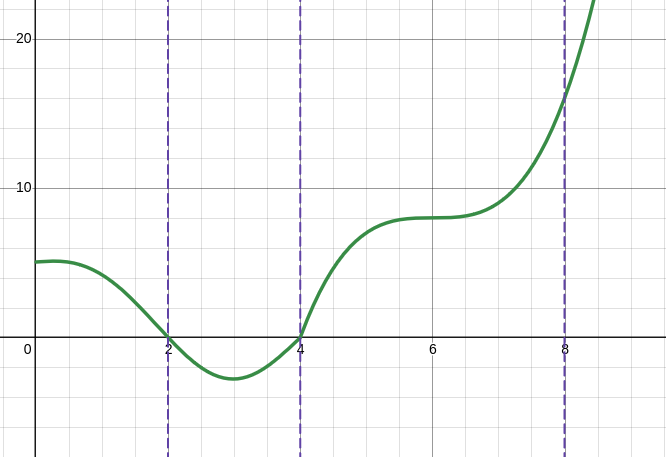
\includegraphics[width=3in]{numeric-integral.png}

	The graph above is of the function $f$. Marked on the graph are the intervals
	$A=[0,2]$, $B=[2,4]$, and $C=[4,8]$. We are interested in the quantity $\displaystyle I=\int_0^8 f(x)\,\mathrm d x$.
	\begin{parts}
		\item On each interval, identify whether left/right/midpoint/trapezoid approximations will produce an
		\begin{enumerate}
			\item Underestimate
			\item Overestimate
			\item Cannot be determined
		\end{enumerate}

		\item Is there any interval where you're confident that Simpson's rule would produce
		an over/under estimate?

		\item Come up with a strategy (i.e., a choice of integration method for each interval)
		that gives the best possible upper and lower bounds for $I$.

	\end{parts}
\end{slide}

\begin{slide}
	\question
	Given an interval $[a,b]$ the midpoint-rule (with one interval) says to use $(b-a)f(0.5a+0.5b)$ as an estimate
	for $I=\displaystyle \int_a^b f(x)\,\mathrm d x$.

	A \emph{biased} midpoint rule with bias $\alpha\in[0,1]$ uses $(b-a)f(\alpha a+(1-\alpha)b)$
	as an estimate for $I$.

	\begin{parts}
		\item Is there a bias $\alpha$ so that with a single partition, $\displaystyle\int_0^1 x^2\,\mathrm d x$ is \emph{perfectly} approximated? If so, what is the bias?

		\item Is there a bias $\alpha$ so that with \emph{two} partitions, $\displaystyle \int_0^1 x^2\,\mathrm d x$ is \emph{perfectly} approximated? If so, what is the bias?

		\item How do your biases compare with the standard midpoint rule?
	\end{parts}
\end{slide}

\begin{slide}
	\question

	\begin{parts}
		\item Explain to your table: What is the difference between a sequence and a series?
		\item How can you produce a sequence from a series?
		\item How can you produce a series from a sequence?
		\item Give an example of a bounded sequence that when summed produces an unbounded series.
	\end{parts}
\end{slide}

\begin{slide}
	\question
	Define the sequence $a_n$ by $
		a_n = \sin(\pi n)$
	and the function $f$ by $f(x) = \sin(\pi x)$.

	\begin{parts}
		\item Find $\displaystyle \lim_{n\to\infty} a_n$, if it exists.
		\item Find $\displaystyle \lim_{x\to\infty} f(x)$, if it exists.

		\item What is the difference between a sequence and a function.
	\end{parts}
\end{slide}

\begin{slide}
	\question
	Define \[
		a_n = \frac{4+n}{2+n} \qquad b_n = \frac{(-1)^n}{n^2}
	\]
	for $n\geq 1$.

	\begin{parts}
		\item If $a_n$ and $b_n$ define sequences, what values can $n$ take on? (E.g., any number in $\R$, any number in $\Z$, etc.)
		\item Make a plot of $a_n$ vs. $n$ and $b_n$ vs. $n$.
		\item Which sequences (out of $a_n$ and $b_n$) are (i) bounded above, (ii) bounded below,
		(iii) strictly increasing, (iv) strictly decreasing, (v) alternating.

		\item Define $c_n=a_{n-1} + b_{2n}$ for $n\geq 2$. Find a formula for $c_n$.

		\item Based on your answer to Part 3, will $c_n$ be bounded above or below?	Neither?

		\item Find $\displaystyle \lim_{n\to\infty} c_n$.
	\end{parts}
\end{slide}

\begin{slide}
	\question
	Let $a_n$ (for $n\geq 1$) be a sequence and define
	\[
		S_n = \sum_{i=1}^n a_n.
	\]
	Let $S_\infty = \lim_{n\to\infty } S_n$.

	\begin{parts}
		\parbox{\textwidth}{
			\item Which of the following statements must be true?

			\begin{enumerate}
				\item If $|a_n| \geq 1$ for all $n$, then $S_n$ converges.
				\item If $|a_n| \leq 1$ for all $n$, then $S_n$ converges.
				\item If $|S_n| \geq 1$ for all $n$, then $a_n$ diverges.
				\item If $|S_n| \leq 1$ for all $n$, then $a_n$ diverges.
				\item If $a_n\to 0$ then $S_n$ converges.

			\end{enumerate}
		}

		\bigskip
		\bigskip
		\item If you switch \emph{converges} $\leftrightarrow$ \emph{diverges},
		which statements change their truth value? (I.e., switch from being true to false or
		false to true.)
	\end{parts}
\end{slide}

\begin{slide}
	\question
	Consider the function $f(x)=1/x$, the sequence $a_n=1/n$ and
	the sequence of partial sums $\displaystyle S_n = \sum_{i=1}^n a_i$.

	In this question we want to get bounds on the \emph{series}
	\[
		\sum_{i=1}^\infty a_i
	\]
	\begin{parts}
		\item Use $\Sigma$-notation to write down a formula for the left-endpoint approximation of
		$\displaystyle \int_1^n \frac{1}{x}\,\mathrm d x$ using a partition
		whose intervals are width $1$.

		\bigskip
		\bigskip
		\bigskip
		\item Use $\Sigma$-notation to write down a formula for the right-endpoint approximation of
		$\displaystyle \int_1^n \frac{1}{x}\,\mathrm d x$ using a partition
		whose intervals are width $1$.
		\item Use the actual value of $\displaystyle \int_1^n \frac{1}{x}\,\mathrm d x$ to give upper and lower bounds for $S_n$.
		\item Does $S_n$ converge or diverge? Explain.
	\end{parts}
\end{slide}

\begin{slide}
	\question
	Consider the function $f(x)=1/x^2$, the sequence $a_n=1/n^2$ and
	the sequence of partial sums $\displaystyle S_n = \sum_{i=1}^n a_i$.

	In this question we want to get bounds on the \emph{series}
	\[
		\sum_{i=1}^\infty a_i
	\]
	\begin{parts}
		\item Use $\Sigma$-notation to write down a formula for the left-endpoint approximation of
		$\displaystyle \int_1^n \frac{1}{x^2}\,\mathrm d x$ using a partition
		whose intervals are width $1$.

		\bigskip
		\bigskip
		\bigskip
		\item Use $\Sigma$-notation to write down a formula for the right-endpoint approximation of
		$\displaystyle \int_1^n \frac{1}{x^2}\,\mathrm d x$ using a partition
		whose intervals are width $1$.
		\item Use the actual value of $\displaystyle \int_1^n \frac{1}{x^2}\,\mathrm d x$ to give upper and lower bounds for $S_n$.
		\item Does $S_n$ converge or diverge? Explain.
		\item Conjecture about the convergence of $\displaystyle \sum_{i=1}^\infty i^{\alpha}$ for $\alpha> 0$. Can you justify your answer by comparing with known integrals?
	\end{parts}
\end{slide}

\begin{slide}
	\question
	Let
	\[
		a_n =\frac{1}{\sqrt{n}}\qquad b_n=\frac{1}{n^3}\qquad c_n=e^{-n}
		\qquad d_n=e^{-n^2}
	\]
	and consider the corresponding sequences of partial sums $A_n$, $B_n$,
	$C_n$, and $D_n$. (I.e., $\displaystyle A_n=\sum_{i=1}^n a_n$, etc.)

	\begin{parts}
		\item Use a comparison with known integrals to decide
		the convergence of $A_n$, $B_n$, $C_n$.
		\item Can you decide the convergence of $D_n$ using a comparison to
		a known integral? Explain.
	\end{parts}
\end{slide}

\begin{slide}
	\question
	Consider the function $f(x)=\sin(x)$.

	\begin{parts}
		\item Write down $T_k(x)$, the $k$th Taylor approximation to
		$f$ centered at $0$. You may use ``$\cdots$'' notation or $\Sigma$-notation.

		\item Write down, using $\Sigma$-notation, $T(x)$, the Taylor series
		for $f$ centered at $0$.

		\item In general a Taylor series may be written as $\displaystyle
			\sum_{n=0}^\infty a_n \frac{x^{n}}{n!}$, where $a_n$ is a sequence.
		Find $a_n$ in this case.

		\item Let $R_k(x)=f(x)-T_k(x)$. Find an expression for $R_k(x)$
		using Taylor's Remainder Theorem. Use your expression to find an upper bound for $|R_k(x)|$ (Hint: your bound may depend on $x$).

		\item Using the fact that for any $\alpha\in \R$,
		$\displaystyle \lim_{n\to\infty} \frac{\alpha^n}{n!}=0$,
		find $\displaystyle \lim_{k\to\infty} R_k(x)$.

		\item For which $x$ is $f(x)=T(x)$? Justify your answer.
	\end{parts}
\end{slide}

\begin{slide}
	\question
	Consider the function $g(x)=\frac{1}{1-x}$. The $k$th Taylor approximation
	of $g$ centered at $0$ is
	\[
		T_k(x)=\sum_{i=0}^k x^k
	\]
	and the remainder $R_k(x)=g(x)-T_k(x)$ satisfies
	\[
		|R_k(x)| \leq \frac{1}{1-x}\left(\frac{x}{1-x}\right)^{k+1}
	\]
	when $x\geq 0$ and
	\[
		|R_k(x)| \leq x^{k+1}
	\]
	when $x< 0$.

	\bigskip
	\bigskip
	\bigskip
	\begin{parts}
		\item For which $x$ is $\lim_{k\to\infty}R_k(x)=0$?

		\item Let $T(x)$ be the Taylor series for $g$ centered at $0$.
		For which $x$ can you guarantee that $g(x)=T(x)$?

		\item Use the following Desmos link to numerically answer the question: for which $x$ does $g(x)=T(x)$?

		{\small\url{https://www.desmos.com/calculator/yi4qczkxqn}}

		\item Does your answer to the previous part contradict Taylor's remainder theorem?

	\end{parts}
\end{slide}

\begin{slide}
	\question
	Let $f(x)=\sin(x)$ and let
	\[
		T(x)=\sum_{n=0}^\infty (-1)^{n}\frac{x^{2n+1}}{(2n+1)!}
	\]
	be the Taylor series for $f$ centered at $0$. We know that
	$f(x)=T(x)$ for all $x\in \R$.

	\begin{parts}
		\item Find a series representation for $g_1(x)=f(2x)$ (without
		computing any derivatives).
		\item Find a series representation for $g_2(x)=f(x^2)$.
		\item Use WolframAlpha to integrate $g_2$. Does WolframAlpha's solution make sense?
		\item Compute $g_3(x)=\displaystyle \int g_2(x)\,\mathrm d x$ by integrating your series for $g_2(x)$ term by term. What should you do with the constants of integration?
		\item For which $x$ do you expect $g_3(x)$ to be valid? Explain.
		\item When would it be advantageous to integrate a Taylor series term by term instead of integrating the original function? Explain.
	\end{parts}
\end{slide}

\begin{slide}
	\question
	Let $f(x)=\frac{1}{1-x}$ and let
	\[
		T(x)=\sum_{n=0}^\infty x^n
	\]
	be the Taylor series for $f$ centered at $0$. We know that
	$f(x)=T(x)$ for all $x\in (-1,1)$.

	\begin{parts}
		\item Find a series representation for $g_1(x)=f(2x)$ (without
		computing any derivatives).
		\item For which $x$ do you expect your series for $g_1(x)$ to be valid (i.e. to equal
		$f(2x)$? Explain.
		\item Find a series representation for $g_2(x)=f(x^2)$.
		\item Compute $g_3(x)=\displaystyle \int g_2(x)\,\mathrm d x$ by integrating your series for $g_2(x)$ term by term.
		\item For which $x$ do you expect $g_3(x)$ to be valid? Explain.
	\end{parts}
\end{slide}

\begin{slide}
	\question
	The function $f$ has a Taylor series centered at $0$ of the form
	\[
		T(x)=-\frac{1}{2}+\frac{x}{3}-\frac{x^2}{4}+\frac{x^3}{5}-\frac{x^4}{6}+\cdots.
	\]

	\begin{parts}
		\item Express $T$ using $\Sigma$-notation.
		\item Find a series representation for $f'(x)$ and $\displaystyle\int f(x)\,\mathrm d x$.
		\item Modify the following Desmos link and make a conjecture: for
		which values of $x$ is $f(x)=T(x)$?

		\url{https://www.desmos.com/calculator/try63qzvo5}

		\item Based on your conjecture, for which values of $x$ should your series for $f'(x)$ and $\displaystyle \int f(x)\,\mathrm d x$ be
		valid?
	\end{parts}
\end{slide}

\begin{slide}
	\question
	Recall
	\[
		\sin x = \sum_{n=0}^\infty (-1)^n\frac{x^{2n+1}}{(2n+1)!}
		\qquad
		\cos x = \sum_{n=0}^\infty (-1)^n\frac{x^{2n}}{(2n)!}
	\]
	for all $x\in\R$.

	Let $f(x)=\cos(\sqrt{x})$.

	\begin{parts}
		\item Write down a Taylor series, $T$, for $f$.

		\emph{Hint: you don't need to take any derivatives.}

		\item Find $f^{(6)}(0)$.

		\item For what $x$ is $T(x)=f(x)$? Explain.

		\item Using Desmos, make a conjecture: for which values of $x$ does your series converge?

		{\small\url{https://www.desmos.com/calculator/try63qzvo5}}

		\item Let $T$ be a Taylor series for an unknown function $g$.
		If $T$ converges at a value $x_0$, must it be true that $T(x_0)=g(x_0)$?
		Explain.

	\end{parts}
\end{slide}


\begin{slide}
	\question%
	\label{geomseq}
	The sequence $a_n$ is defined by $a_0=10$ and
	\[
		\frac{a_{n+1}}{a_n}= \frac{1}{4}
	\]

	Define $\displaystyle S_n=\sum_{i=0}^n a_i$ and
	$\displaystyle S=\lim_{n\to\infty} S_n$.

	\begin{parts}
		\item  Find an expression for $a_n$.
		\item Is $S_n$ bounded? Explain.
		\item Compute $S$.

		\emph{Recall:
			$\displaystyle
				\sum_{i=0}^n \alpha^i = \frac{1-\alpha^{n+1}}{1-\alpha}
			$}

	\end{parts}
\end{slide}

\begin{slide}
	\question
	Recall the sequence $a_n$ from Exercise \ref{geomseq} defined by
	$a_0=10$ and
	$\displaystyle
		\frac{a_{n+1}}{a_n}= \frac{1}{4}
	$.

	Consider the unknown, positive, sequence $b_n$. You know that $b_0=5$ and
	$\displaystyle \frac{b_{n+1}}{b_n} < \frac{1}{5}$.

	\begin{parts}
		\item Do you have enough information to write down an expression for $b_n$?

		\item Which (if any) of the following relationships must hold for all $n$?
		\[
			a_n < b_n \qquad b_n < a_n \qquad a_n = b_n
		\]
		Justify your answer.

		\item Consider the series $\displaystyle \sum_{n=0}^\infty
			b_n$. Does the series converge? Justify your answer by comparing with
		a known series.

		\item If you were told that, actually, $b_0=100$, would that
		change your answer to the previous part?
	\end{parts}

\end{slide}
\begin{slide}
	\question
	The ratio test states for a sequence $c_n$ if
	\[
		\lim_{n\to\infty} \frac{|c_{n+1}|}{|c_n|} < 1
	\]
	then $\displaystyle \sum_{n=0}^\infty c_n$ converges.

	Recall the sequence $a_n$ from Exercise \ref{geomseq} defined by
	$a_0=10$ and
	$\displaystyle
		\frac{a_{n+1}}{a_n}= \frac{1}{4}
	$.

	You know the following about the positive sequence $d_n$:
	$\displaystyle \lim_{n\to\infty} \frac{d_{n+1}}{d_n} =\rho < \frac{1}{5}$.

	\begin{parts}
		\item Which (if any) of the following relationships must hold for all $n$?
		\[
			a_n < d_n \qquad d_n < a_n \qquad a_n = d_n
		\]
		\item Which (if any) of the following relationships \emph{eventually} hold (i.e. hold for all sufficiently large $n$)?
		\[
			a_n < d_n \qquad d_n < a_n \qquad a_n = d_n
		\]
		Justify your answer.

		\item Justify, without the ratio test, whether $\displaystyle
			\sum_{n=0}^\infty d_n$ converges.

		\item Prove the ratio test.
	\end{parts}
\end{slide}

\begin{slide}
	\question
	\begin{theorem}[(Ratio Test)]
		If $c_n$ is a sequence and
		\[
			\lim_{n\to\infty} \frac{|c_{n+1}|}{|c_n|} =\rho
		\]
		then $\displaystyle \sum_{n=0}^\infty c_n$

		\begin{itemize}
			\item converges if $\rho < 1$
			\item diverges if $\rho > 1$
			\item could converge or diverge if $\rho =1$
		\end{itemize}
	\end{theorem}

	\begin{parts}
		\item
		\begin{minipage}[t]{0.45\textwidth}
			The Ratio Test talks about the convergence of $\displaystyle \sum_{n=0}^\infty c_n$.
			Does it also apply to sums that don't start at $n=0$? Explain.
		\end{minipage}
		\item Apply the ratio test to determine the convergence of the
		following series:
		\begin{enumerate}
			\item $\displaystyle \sum_{n=1}^\infty \frac{2^{n}}{n!}$
			\item $\displaystyle \sum_{n=1}^\infty \frac{8^n}{(-2)^{n+1}n}$
			\item $\displaystyle \sum_{n=1}^\infty \frac{1}{n}$
		\end{enumerate}
	\end{parts}
\end{slide}

\begin{slide}
	\question
	The Taylor series for $f(x)=\frac{1}{1-2x}$ is
	\[
		T(x)=\sum_{n=0}^\infty 2^nx^n
	\]

	\begin{parts}
		\item Apply the ratio test to $T(x)$. Does $T(x)$ converge?
		Does your answer depend on $x$?
		\item Let $G(x)$ be the Taylor series for $g(x)=e^x$. Apply the ratio
		test to $G(x)$. Does your answer depend on $x$?
		\item Write down the largest (open) interval of convergence and the radius of convergence for $T$ and $G$.
	\end{parts}
\end{slide}

\begin{slide}
	\question
	The Taylor series for $h(x)=\frac{1}{1-x}$ centered at $a>1$ is
	\[
		H(x)=\sum_{n=0}^\infty \frac{(x-a)^n}{(1-a)^{n+1}}.
	\]


	\begin{parts}
		\item Find the largest (open) interval of converge and radius of convergence for $H$.
		\item Graph $h$. Just looking at the graph, can you determine
		whether a Taylor series for $h$ should have an infinite or finite radius of converge?
	\end{parts}
\end{slide}



\begin{slide}
	\question

	\begin{theorem}[(Integration by Parts)]
		If $f(x)$ and $g(x)$ are differentiable functions, then
		\[
			\int f(x)g'(x)\,\mathrm d x
			= f(x)g(x) -
			\int f'(x)g(x)\,\mathrm d x
		\]
	\end{theorem}

	\begin{parts}
		\item The integration by parts formula comes from reversing
		one of the differentiation rules (e.g., chain rule/product rule/quotient rule). Which rule does the integration by parts formula come from?
		\item
		Let $h_1(x)=x\sin x$.

		\begin{enumerate}
			\item
			      For $h_1$, write down all the ways to divide it into
			      a product of  ``parts'' $f$ and $g'$ so that $h_1=f\cdot g'$.
			\item Pick the decomposition into parts that you think will be most useful and integrate $h_1$.
		\end{enumerate}

		\item
		Let $h_2(x)=x^3 e^{x^2}$.
		\begin{enumerate}
			\item
			      For $h_2$, write down all the ways to divide it into
			      a product of  ``parts'' $f$ and $g'$ so that $h_2=f\cdot g'$.
			\item Pick the decomposition into parts that you think will be most useful and integrate $h_2$.
		\end{enumerate}

	\end{parts}
\end{slide}


\begin{slide}
	\question

	\begin{theorem}[(Integration by Parts)]
		If $f(x)$ and $g(x)$ are differentiable functions, then
		\[
			\int f(x)g'(x)\,\mathrm d x
			= f(x)g(x) -
			\int f'(x)g(x)\,\mathrm d x
		\]
	\end{theorem}

	\begin{parts}
		\item Use integration by parts to find $\displaystyle \int e^x\sin x\,\mathrm d x$.

		Hint: \emph{if at first you don't succeed, try, try again.}

		\item Use integration by parts to find $\displaystyle \int_1^2 \ln x\,\mathrm d x$.

		Hint: \emph{sometimes $g$ is hiding in plain sight.}
	\end{parts}
\end{slide}


% \begin{slide}
% 	\question

% 	\begin{minipage}{\textwidth}
% 	For each integral, decide whether you would use integration by
% 	parts. If you would, describe the parts.


% 	\begin{center}
% 	\renewcommand{\arraystretch}{2.5}
% 	\begin{tabular}{|c|c|c|}
% 		\hline 
% 		Integral & $\phantom{x}\qquad f=?$\qquad $g=?$\qquad \phantom{x}& Other method? \\
% 		\hline 
% 		$\displaystyle \int xe^{2x-3}\,\mathrm d x$ &&\\[6pt]
% 		 \hline
% 		$\displaystyle \int t^3e^{t^3}\,\mathrm d t$ &&\\[6pt]
% 		 \hline
% 		$\displaystyle \int \sin(\ln x)\,\mathrm d t$ &&\\[6pt]
% 		 \hline
% 		$\displaystyle \int x^2\sin(t)\,\mathrm d t$ &&\\[6pt]
% 		 \hline
% 	\end{tabular}
% 	\end{center}
% 	\end{minipage}

% \end{slide}



\begin{slide}
	\question
	We would like to compute
	\[
		F(\theta) = \int \sin^2(\theta)\,\mathrm d \theta
	\]

	\begin{parts}
		\item (Review) Use integration by parts to find $F(\theta)$.

		Hint: \emph{The identity $1=\cos^2\theta +\sin^2\theta$ may reduce your workload.}

		\item Use the trig identity $\displaystyle\sin^2\theta = \frac{1-\cos 2\theta}{2}$
		to find $F(\theta)$.

		\item Find $\displaystyle \int \cos^2(\theta)\,\mathrm d \theta$ using any method you like.
	\end{parts}
\end{slide}

\begin{slide}
	\question
	\label{qtrigsub1}
	Let $f(x)=\sqrt{1-x^2}$ and consider
	\[
		I=\int_0^1 f(x)\,\mathrm d x
	\]

	\begin{parts}
		\item If we define a change of variables $x=\sin \theta$, what would
		$\mathrm d x$ equal?
		\item Apply the substitution $x=\sin\theta$ to get a new function
		$g(\theta)$ so that
		\[
			\int_0^1 f(x)\,\mathrm d x
			=
			\int_?^? g(\theta)\,\mathrm d \theta
		\]

		Find the function $g$ and the bounds for the new integral (i.e. fill in the $?$'s).

		\item Find $I$.

		\item Graph $f$. What shape does the graph make? Use your knowledge
		of geometry to find $I$.
	\end{parts}
\end{slide}

\begin{slide}
	\question
	In Exercise \ref{qtrigsub1} we computed
	\[
		I=\int_0^1 \sqrt{1-x^2}\,\mathrm d x = \int_0^{\pi/2} \cos^2\theta\,\mathrm d \theta
	\]

	\begin{parts}
		\item Explain why the bounds changed from $[0,1]$ to $[0,\pi/2]$.
		\item Would it be okay to change the bounds from $[0,1]$ to $[2\pi, 5\pi/2]$?
		\item Would it be okay to change the bounds from $[0,1]$ to $[0, 5\pi/2]$?
		\item Compute $I$ using the substitution $x=\cos\theta$. Pay close attention to
		make sure you use the correct bounds.
	\end{parts}
\end{slide}



\begin{slide}
	\question
	Let $\displaystyle f(x)=\frac{\sqrt{9-x^2}}{x^2}$ and consider
	\[
		F(x)=\int f(x)\,\mathrm d x
	\]
	Using a substitution of $x=3\sin\theta$,  we arrive at
	\[
		F(x)=-\frac{\cos\theta}{\sin\theta} - \theta + C.
	\]

	\begin{parts}
		\item Find an expression for $F(x)$ that involves only $x$.
		\item Are there restrictions on domain of $x$ for which your
		answer makes sense?
		\item The domain of $\arcsin$ is $[-1,1]$. Does this change your
		restrictions on the domain of $x$?
	\end{parts}
\end{slide}


\begin{slide}
	\question
	Let $\displaystyle f(x)=\sqrt{\cos x}$ and consider
	\[
		I=\int_0^{\sqrt{2}} f(x)\,\mathrm d x
	\]

	You would like to find $I$.
	\begin{parts}
		\item Use WolframAlpha to find an anti-derivative of $f$.
		Does WolframAlpha give you a useful answer?
		\item Using a 2$^{\text{nd}}$ degree Taylor approximation for $\cos$,
		write down an integral that will approximate $I$.
		\item Find an approximation for $I$.
		\item Use a 2$^{\text{nd}}$ degree Taylor approximation for $f$ to
		approximate $I$.
		\item Desmos claims $I\approx 1.15686930348$. Which of your estimates is more accurate?

	\end{parts}
\end{slide}


\begin{slide}
	\question
	Let
		\[
			f(x)=\frac{1}{x^2-1}\qquad
			\text{and}
			\qquad g(x)=\frac{A}{x-1}+\frac{B}{x+1}.
		\]

	\begin{parts}
		\item
		You would like to know if
		there are constants $A$ and $B$ such that $f(x)=g(x)$ for all $x$.

		Set up a system of linear equations (or a matrix equation) which has a
		solution if and only if there are constants $A$ and $B$ that make $f(x)=g(x)$ for all $x$ (in the domain of $f$).
		\item Find $A$ and $B$, if possible.
		\item Compute $\displaystyle \int f(x)\,\mathrm d x$ using any method of your choice.
	\end{parts}
\end{slide}

\begin{slide}
	\question
	Let
		\[
			f(x)=\frac{1}{(x-1)x^2}\qquad
			\text{and}
			\qquad g(x)=\frac{A}{x-1}+\frac{B}{x}.
		\]

	\begin{parts}
		\item
		You would like to know if
		there are constants $A$ and $B$ such that $f(x)=g(x)$ for all $x$.

		Set up a system of linear equations (or a matrix equation) which has a
		solution if and only if there are constants $A$ and $B$ that make $f(x)=g(x)$ for all $x$ (in the domain of $f$).
		\item Find $A$ and $B$, if possible.
		\item Let $h(x)=\frac{A}{x-1}+\frac{B}{x}+\frac{C}{x^2}$. Can you find 
		constants $A$, $B$, and $C$ so that $f(x)=h(x)$ for all $x$ (in the domain of $f$)? If so, do it.
		\item Compute $\displaystyle \int f(x)\,\mathrm d x$ using any method of your choice.
	\end{parts}
\end{slide}

\begin{slide}
	\question
	We know $\int \frac{1}{x^2+1}\,\mathrm d x = \arctan x + C$. However, we can 
	also use partial fraction decomposition over the complex numbers to integrate.

	Let $f(x)=\frac{1}{1+x^2}$ and $g(x)=\frac{A}{1+ix}+\frac{B}{1-ix}$.

	\begin{parts}
		\item Find $A$ and $B$ so that $f(x)=g(x)$ for all $x$ (in the domain of $f$).
		\item Compute $\displaystyle \int f(x)\,\mathrm d x$ using your result from the previous part.

		\emph{However:} use $\ln x$ as the antiderivative of $\frac{1}{x}$ rather
		than $\ln |x|$.
		\item Use the fact that $\ln (re^{i\theta})=\ln r + i\theta$ to simplify your answer.
	\end{parts}
\end{slide}


\begin{slide}
	\question
	An \emph{improper integral} formalizes the concept of the area 
	under an ``infinite'' curve.

	Suppose $f$ is a bounded function and let $\displaystyle I=\int_0^\infty f(x)\mathrm d x$.

	\begin{parts}
		\item Write down a formal definition of $I$.
		\item Compute, using the definition, 
		$\displaystyle \int_0^\infty \frac{1}{(x+1)^2}\mathrm d x$
		\item Compute, using the definition, 
		$\displaystyle \int_0^\infty \frac{1}{(x+1)}\mathrm d x$
	\end{parts}
\end{slide}

\begin{slide}
	\question
	Let $\displaystyle f(x)=\frac{x}{x^2+1}$

	In this question, we will try to compute
	\[
	Q=\int_{-\infty}^\infty f(x)\,\mathrm d x
	\]

	\begin{parts}
		\item Graph $f$. Make a guess on what you think the ``total area under the curve'' (i.e. $Q$) should be.
		\item Find $\displaystyle \int f(x)\,\mathrm d x$
		\item Compute $
		\displaystyle 
		\lim_{N\to\infty} \int_{-N}^N f(x)\,\mathrm d x
		$. Should your result be equal to $Q$?
		\item Should $
		\displaystyle 
		\lim_{N\to\infty} \int_{-N}^{2N} f(x)\,\mathrm d x
		$ correspond to $Q$? Compute it and compare with the previous part.

		\item Compute $A=\displaystyle \int_0^\infty f(x)\,\mathrm d x$
		and $B=\displaystyle \int_{-\infty}^0 f(x)\,\mathrm d x$.

		\item By the properties of integrals, we must have
		\[
			Q=A+B.
		\]
		Do the properties of integrals hold for this improper integral?
		What does this say about $Q$?
	\end{parts}
\end{slide}

\begin{slide}
	\question
	The moral of improper integral is:
	\begin{quote}
		\emph{Wherever an infinity might appear, take a separate limit.}
	\end{quote}

	\begin{parts}
		\item Rewrite 
		$\displaystyle \int_{-\infty}^\infty \frac{x}{x^2+1}\,\mathrm d x$
		using limits of definite integrals.
		\item Let $g(x)=\frac{1}{x^{1/3}}$ and consider 
		$I=\displaystyle \int_{-8}^{27} g(x)\,\mathrm d x$.

		\begin{enumerate}
			\item Identify all regions where $\displaystyle \int g(x)\,\mathrm d x$ \emph{could} produce infinities.
			\item Rewrite $I$ using limit(s) of definite integrals.
			\item Find $I$.
		\end{enumerate}
	\end{parts}

\end{slide}

\begin{slide}
	\question

	Let $\displaystyle f(x)=\frac{\ln|x|}{x^4+1}$
	\[
	J=\int_{-\infty}^\infty f(x)\,\mathrm d x
	\]

	\begin{parts}
		\item Rewrite $J$ using limit(s) of definite integrals.
		\item 
		Consider the functions
		\[
			b_1(x)=\ln x \qquad b_2(x)=\frac{\ln x}{2}
		\]
		\[
			b_3(x) = \frac{x}{x^4+1}\qquad b_4(x)=0
		\]
		\begin{enumerate}
		\item Let $A=\displaystyle \int_0^1 f(x)\,\mathrm d x$.
		Find upper and lower bounds for $A$ by comparing with the
		appropriate $b_?$ 
		functions.

		\item Let $B=\displaystyle \int_1^\infty f(x)\,\mathrm d x$.
		Find upper and lower bounds for $B$.

		\end{enumerate}
		
		\item Use your results from the previous part to find upper and lower bounds for $J$.
		
	\end{parts}
\end{slide}

\begin{slide}
	\question

	Consider the functions
	\[
		A(t)=t \qquad B(t)=t^2 \qquad C(t)=t^{1/2}
	\]
	\[
		D(t)=2t \qquad E(t)=2t^2 \qquad F(t)=2t^{1/2}
	\]

	\begin{parts}
		\item Consider the parametric equations $x(t)=A(t)$ and $y(t)=D(t)$.

		Graph, by hand, $(x,y)$ for $t\in [0,4]$.

		\item Consider the parametric equations $x(t)=B(t)$ and $y(t)=A(t)$.

		Graph, by hand, $(x,y)$ for $t\in [0,4]$.

		\item Identify all possible assignments of $x(t)=\,??$ and $y(t)=\,??$ 
		(where $??$ come from the functions above) so that 
		the graph of $(x,y)$ for $t\in [0,4]$ is a line segment.

		\item Out of your examples above, which example produces the \emph{longest} line segment?
		
	\end{parts}
\end{slide}

\begin{slide}
	% https://www.desmos.com/calculator/bf4a7hrudl
	\question

		Show is the graph of $\displaystyle
		\begin{cases}
			x(t)=3\cos t \\
			y(t)=t^2-5t
		\end{cases}
		$
		for $t\in[0,2\pi]$.
		\begin{center}
	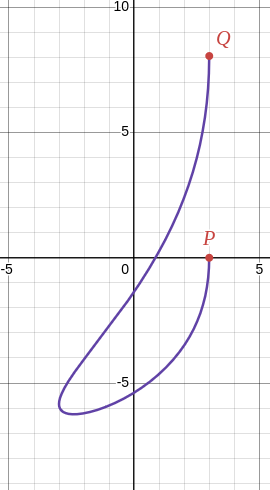
\includegraphics[height=2in]{images/parametric1.png}
		\end{center}

	
	The parametric equations describe the position of a particle at time $t$.

	\begin{parts}
		\item Is the particle moving from $P$ to $Q$ or $Q$ to $P$? Explain.

		\item At what time(s) is the particle moving up \emph{and} to the right?

		\item At what time(s) is the particle moving parallel to the $x$-axis?

		\item Find the tangent line to the particles path at time $t=\pi/2$.
		
	\end{parts}
\end{slide}


\begin{slide}
	% https://www.desmos.com/calculator/bf4a7hrudl
	\question

		Show is the graph of $\displaystyle
		\begin{cases}
			x(t)=3\cos t \\
			y(t)=t^2-5t
		\end{cases}
		$
		for $t\in[0,2\pi]$.
		\begin{center}
	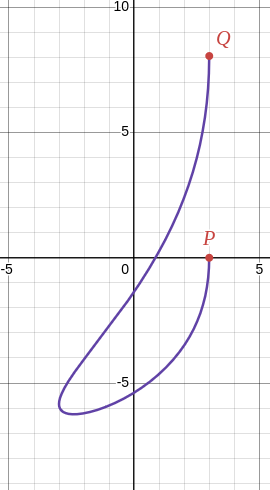
\includegraphics[height=2in]{images/parametric1.png}
		\end{center}

	
	The parametric equations describe the position of a particle at time $t$.

	\begin{parts}
		\item Find a parameterization for a particle that traces the same path,
		but starts at $Q$ and ends at $P$.

		\item Find a parameterization so that the particle finishes its journey in $\pi$ seconds instead of $2\pi$ seconds.

		\item Is there a parameterization so that the particle
		finishes its journey in $\pi$ seconds but starts its journey at
		the same speed as the original particle? If such a parameterization exists, how would you come up with it?
		
	\end{parts}
\end{slide}


\begin{slide}
	% https://www.desmos.com/calculator/bf4a7hrudl
	\question

		Show is the graph of $\displaystyle
		r(\theta)=\sin(3\theta)
		$
		in polar coordinates
		for $\theta\in[0,\pi]$.
		\begin{center}
	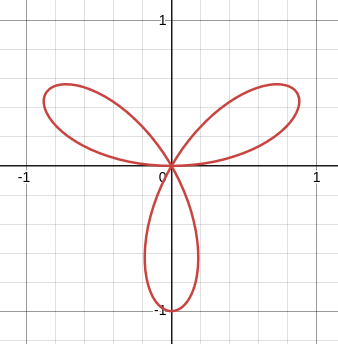
\includegraphics[height=2in]{images/parametric2.png}
		\end{center}

	
	The curve models the boundary of a propeller.

	\begin{parts}
		\item The blade in the first quadrant achieves a maximum length at 
		an angle of $\theta =\pi/6$. Find the rectangular coordinates of
		the tip of the blade in the first quadrant.

		\item Find parametric equations $(x(t), y(t))$ that trace out the 
		propeller.

		\item Find the tangent line to the propeller when $\theta=0$
		and when $\theta =\pi/3$.

		\item We know that the propeller is contained in 
		a circle with area $\pi$.

		Come up with a better upper bound for the area of the 
		propeller.		
	\end{parts}
\end{slide}

\begin{slide}
	% https://www.desmos.com/calculator/agec13lrk2
	\question
		The same semi-circle can be described in polar coordinates by
		\[
r(\theta)=\cos\theta\quad\text{ with }\quad\theta\in[0,\pi/2]
		\]
		 or in rectangular
		coordinates by \[
		y(x)=\sqrt{\tfrac{1}{4}-(x-\tfrac{1}{2})^2}\quad\text{ with }\quad x\in[0,1].
		\]

		Below are two ways to divide up the semicircle to approximate its area: one with rectangles and one with circular \emph{sectors}.
		\begin{center}
	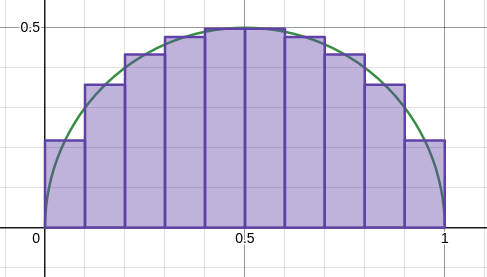
\includegraphics[height=1in]{images/riemann-rect.png}
		\end{center}
		\begin{center}
	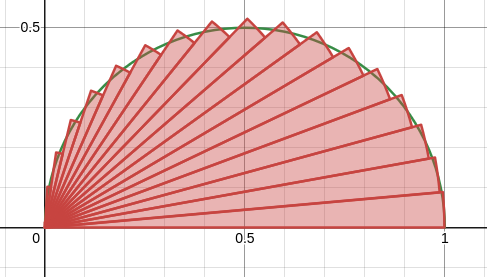
\includegraphics[height=1in]{images/riemann-polar.png}
		\end{center}

	
	\begin{parts}
		\item Write down a Riemann sum that approximates the area using 
		\emph{rectangles}. Use $\Delta x$ as the width of a rectangle.

		\item Write down a Riemann sum that approximates the area using 
		\emph{sectors}. Use $\Delta \theta$ as the sector angle.
		
		\item Take limits of your previous two Riemann sums to find 
		integrals integrals to represent the \emph{exact} area of the semicircle. 

		\emph{Do not evaluate your integrals.}

		\item Which integral would you rather do?
	\end{parts}
\end{slide}

\begin{slide}
	% https://www.desmos.com/calculator/bf4a7hrudl
	\question

		Show is the graph of $\displaystyle
		r(\theta)=\sin(3\theta)
		$
		in polar coordinates
		for $\theta\in[0,\pi]$.
		\begin{center}
	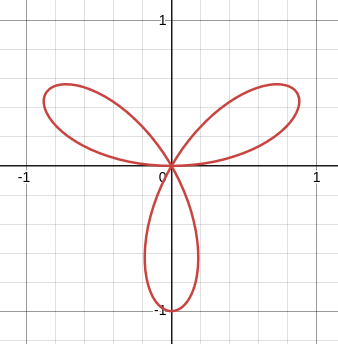
\includegraphics[height=2in]{images/parametric2.png}
		\end{center}

	
	The curve models the boundary of a propeller.

	\begin{parts}
		\item The first propeller blade is traced out for $\theta\in[0,\pi/3]$
		
		Set up a Riemann sum that approximates the area of the first propeller
		blade.

		\item Set up an integral that will give the \emph{exact} area of the
		first propeller blade. Then, find the area of the first propeller blade.

		\item Find the total area of the propeller.
	\end{parts}
\end{slide}


\begin{slide}
	% https://www.desmos.com/calculator/yrzsjkewdc
	\question

		Show is the graph of $\displaystyle
		r(\theta)=\sin(3\theta)
		$
		in polar coordinates
		for $\theta\in[0,\pi]$.
		\begin{center}
	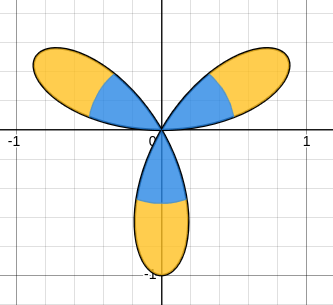
\includegraphics[height=2in]{images/propeller-painted.png}
		\end{center}

	
	The curve models the boundary of a propeller. The parts of the propeller
	within distance $1/2$ of the origin are painted blue. The rest is painted yellow.

	\begin{parts}
		\item Consider the propeller blade in the first quadrant. At what
		angle does the yellow paint start to appear? At what angle does it 
		disappear?

		\item Set up an integral that will give the amount of yellow paint needed for the first blade.

		\item Set up an expression with integral(s) that will give the amount of blue paint needed
		for the first blade.

		\item Find the amounts of each paint needed to paint the 
		whole propeller.
	\end{parts}
\end{slide}



\end{document}
